\section{绪论}
%\pagestyle{plain}
\setcounter{page}{1}%该页页码为第一页
\pagenumbering{arabic}
%\setcounter{page}{1}
%\pagestyle{plain}
\subsection{拓扑绝缘体}
\qquad1980年实验物理学家Kalus von Klitzing在二维电子气中加入高磁场,发现体系的霍尔电阻随着磁场强度改变的时候出现了一些非常平整的平台\cite{re1}。这种整数化的平台其实是量子效应的一种宏观表现,正是这个发现为人们打开了研究拓扑物态的大门,而Kalus von Klitzing也因此获得了1985年的诺贝尔物理学奖。当均匀的电子气处于强磁场的时候会形成Landua能级,如果体系的费米面恰好处于Landua能级的中间,由能带论可知系统此时处于绝缘状态。但是之后的研究却发现虽然在强磁场下体系内部是绝缘的,但是在边界上却形成了无耗散的导电通道,正是这些通道的存在形成了平台化的霍尔电阻。1982年David J. Thouless,J.Michael Kosterlitz等人(TKNN)对这个量子化的平台给出了完美的解释\cite{re2}。通过Kubo公式求解体系霍尔电导发现它和一个正数是相关的,也就是说霍尔电导等于$ne^2/h$,这里的正数$n$表示为:
\begin{equation}	
n=\frac{1}{2}\int_{\mathrm{BZ}}d^2k\nabla_k\times i\sum_{l\in\mathrm{bands}}\langle\varphi_l|\nabla_k|\varphi_l\rangle
\end{equation}
人们将正数$n$称为第一陈数(Chern Number)。从能带论的角度出发进行考虑,陈数代表的是二维电子气系统的一种拓扑性质,在不闭合体系能隙的时候,连续地改变哈密顿量不会引起它的改变,所以被称为拓扑不变量,这个量仅关联与电子态的拓扑性质。把环境与均匀二维电子气当作一个整体,当电子态从电子气体系中演化到环境的时候,陈数将会由非零变为零,那么在环境与电子气的交界处必须存在着一个能隙为零的界面来过渡,这样才可以实现陈数的变化。霍尔电导与陈数之间的这种深刻联系完美解释了霍尔电导量子化平台的起源,也打开了拓扑物态在物理学领域的应用大门。
\begin{figure}
\centering
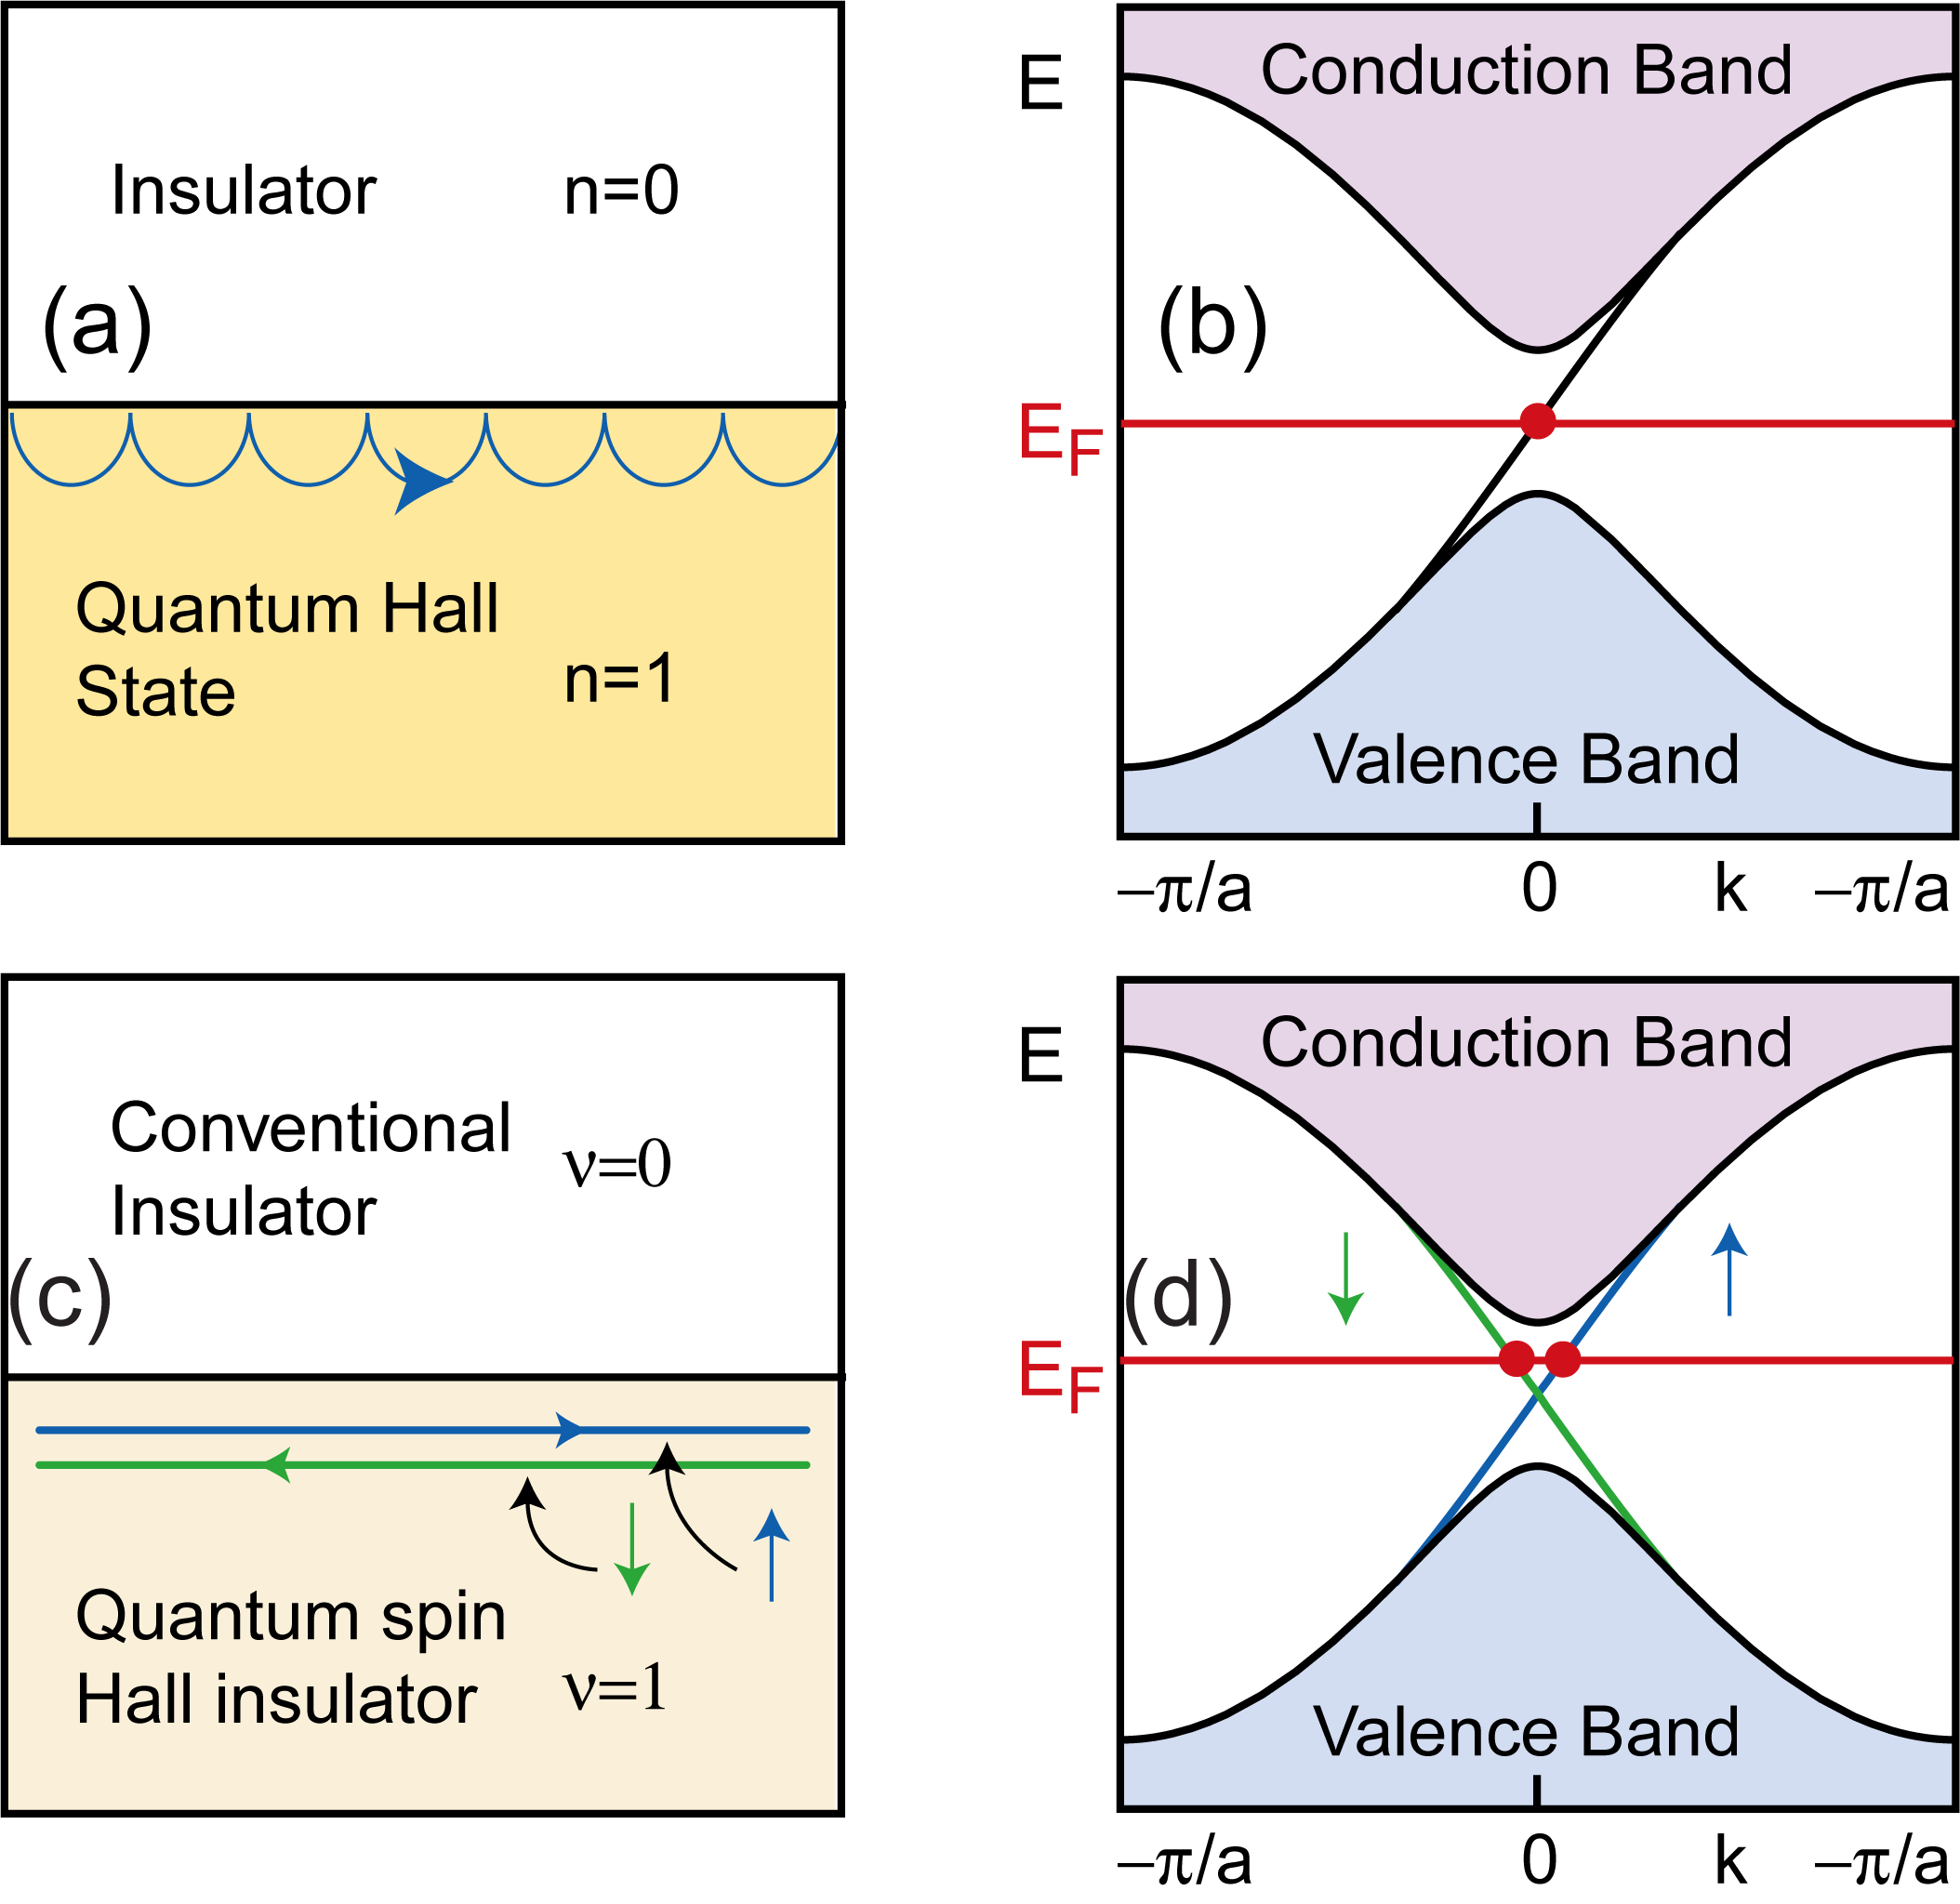
\includegraphics[scale=0.5]{pic/fig1.png}
\caption{(a)整数量子霍尔效应示意图。(b)整数量子霍尔效应能带示意图。(c)整数量子自旋霍尔效应示意图。(b)整数量子自旋霍尔效应能带示意图。}
\end{figure}

%======================================================
\subsection{拓扑超导体}
%======================================================
\subsection{高阶绝缘体}
%======================================================
\subsection{拓扑量子计算}

